\section{Week 6 \& 7: Excitons}
\subsection{Section 1; Model}
\begin{exercise}
We are considering a simple two band model of a one dimensional semi-conductor. The valence and conduction band atomic orbitals of unit cell $n$ are denotes $\phi_{vn}\qty(r) = \phi_v\qty(r- R_N)$ and $\phi_{vn}\qty(r) = \phi_v\qty(r- R_N)$ respectively and satisfy the orthonormality relations, \ie, $\ip{\psi_{n,\alpha}}{\psi_{m,\beta}} = \delta_{nm}\delta{\alpha\beta}$ for $\alpha,\beta \in \{v,c\}$. The non-interacting part of the Hamiltonian takes the form: 
\begin{equation}
    \begin{split}
        H_0 =& \sum_n \varepsilon_v \crea{c}{nv} \anni{c}{nv} + t \qty(\crea{c}{nv} \anni{c}{n+1,v} + \crea{c}{nv}\anni{c}{n-1,v})\\
        +& \sum_n \varepsilon_c \crea{c}{nc} \anni{c}{nc} - t \qty(\crea{c}{nc} \anni{c}{n+1,c} + \crea{c}{nc}\anni{c}{n-1,c})\\
    \end{split}
\end{equation}
Calculate and sketch the band structure assuming that $\varepsilon_c - \varepsilon_v > 4t$. Express the gab in terms of the parameters of the model. Sketch the joint density of states and identify the critical points.
\end{exercise}

\begin{solution}
We let the Hamiltonian act on a Bloch state $\ket{k} = \sum_n e^{ikna} \ket{n}$ and otherwise follow the exact same approach as solution 1.2.2, the first term will only give contributions in the valence band, whereas the second will only give contributions in the conduction band, thereby we have from equation \ref{eq:114} that
\begin{equation}
\begin{split}
    \varepsilon_{valence} = \varepsilon_v + 2t\cos(ka) \\
    \varepsilon_{conduction} = \varepsilon_c - 2t\cos(ka)
    \end{split}
\end{equation}
As $\varepsilon_c - \varepsilon_v > 4t$ there is a bandgap.


\begin{figure}[!ht]
    \centering
    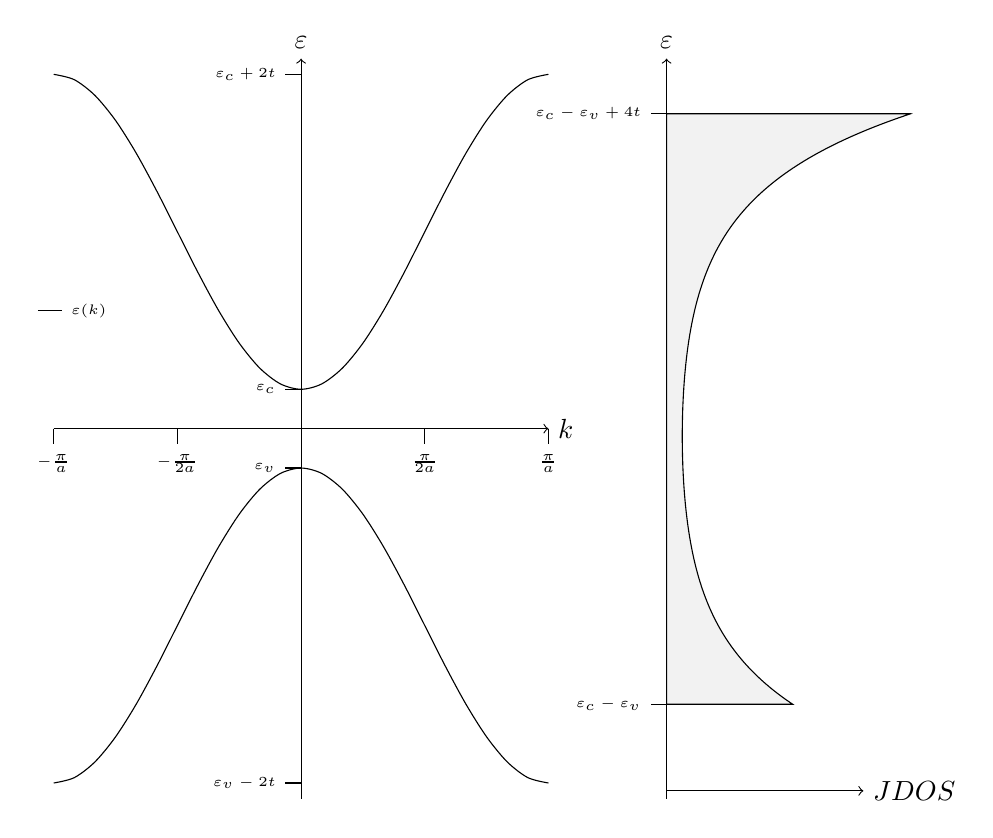
\begin{tikzpicture}
    % Axes
    \draw[->] (-pi,0) -- (pi,0) node[right] {$k$};
    \draw[->] (0,-4.7) -- (0,4.7) node[above] {$\varepsilon$};
    
    % Ticks
        %y
        \draw (0,4.5) -- (-0.2,4.5) node[left] {\tiny{$\varepsilon_c + 2t$}};
        \draw (0,0.5) -- (-0.2,0.5) node[left] {\tiny{$\varepsilon_c$}};
        \draw (0,-0.5) -- (-0.2,-0.5) node[left] {\tiny{$\varepsilon_v$}};
        \draw (0,-4.5) -- (-0.2,-4.5) node[left] {\tiny{$\varepsilon_v-2t$}};
        
        %x
        \draw (-pi,0)   -- (-pi,-0.2)    node[below] {\tiny{$-\frac{\pi}{a}$}};
        \draw (-pi/2,0) -- (-pi/2,-0.2)  node[below] {\tiny{$-\frac{\pi}{2a}$}};
        \draw (pi/2,0)  -- (pi/2,-0.2)   node[below] {\tiny{$\frac{\pi}{2a}$}};
        \draw (pi,0)    -- (pi,-0.2)     node[below] {\tiny{$\frac{\pi}{a}$}};
    
    % Legend
    \draw (-pi-0.2,1.5) -- (-pi+0.1,1.5) node[right] {\tiny{$\varepsilon(k)$}};
    
    
    % Bands
    \draw[color=black,smooth,domain=-pi:pi]  plot (\x,{2.5-2*cos(\x r)});
    \draw[color=black,smooth,domain=-pi:pi]  plot (\x,{-(2.5-2*cos(\x r))});
    
    
    
    % Axes for JDOS
    \draw[->] (pi+1.5,-4.6) -- (pi + 4,-4.6) node[right] {$JDOS$};
    \draw[->] (pi+1.5,-4.7) -- (pi+1.5,4.7) node[above] {$\varepsilon$};
    
    
    %Ticks for JDOS
    \draw (pi+1.5,-3.5) -- (pi+1.3,-3.5) node[left] {\tiny{$\varepsilon_c -\varepsilon_v$}};
    \draw (pi+1.5,4) -- (pi+1.3,4) node[left] {\tiny{$\varepsilon_c -\varepsilon_v + 4t$}};
    
    
    % JDOS
    %\filldraw[color=black,fill=black!5!white,smooth,samples=1000,variable=\y,domain=-3.5:0.5] (pi+1.5,-3.5) -- (pi+2.75,-3.5) -- plot ({pi+1.6+1.15*exp(-(\y+3.5))},{\y}) -- (pi+1.5,4.5) -- (pi+4,4.5);
    \filldraw[color=black,fill=black!5!white,smooth,samples=1000,variable=\y,domain=-3.5:4] (pi+1.5,-3.5) -- (pi+2.75,-3.5) -- plot ({1.5*exp(-(\y+3.5))+pi+1.6+3*exp(-(4-\y))},{\y}) -- (pi+1.6+3,4) -- (pi+1.5,4) -- (pi+1.5,-3.5);
    
\end{tikzpicture}
%{-(1/2)/(sqrt(abs(1-(\y+3.5)*(\y-4.5)/4)))}
    \caption{dispersion relation and DOS of the 1D dimerised chain. Recalling that the short and long latice spacing, $a'$ and $b$ respectively, satisfy $a'+b = 2a$ where $a$ is the latice spacing of the non-dimerized chain.}
    \label{fig:1D_Dimer_Exciton}
\end{figure}

\end{solution}



\subsection{Section 2; Particle-hole excitations}
\begin{exercise}
It turns out that for our purpose it is simpler to represent the states in terms of the atomic orbital basis. Argue that the ground state can be written as
\begin{equation}
    \ket{\Psi_0}  =  \prod_n c_{n,v}^{\dagger} \ket{0}
    \label{eq:groundState}
\end{equation}
\end{exercise}

\begin{solution}
 From equation (6) in the problem handout we see that electrons are added to all states in the FBZ, so it makes sense to add all n states in the FBZ to the zero state.
\end{solution}

\subsection{Section 3; Collective excitations: Excitons}
\begin{exercise}
We now perform a particle-hole transformation by introducing a new set of creation/annihilation operators as
\begin{equation}
    \crea{b}{nv} = \anni{c}{n,v}, \quad \anni{b}{n,v} = \crea{c}{n,v}, \quad \crea{b}{n,c} = \crea{c}{n,c}, \quad \anni{b}{n,c} = \anni{c}{n,c}
\end{equation}
The operators $\crea{b}{}$ create electrons in the conduction band and holes in the valence band. The groundstate $\ket{\Psi_0}$ is the vacuum state for the new operators (denoted by $\ket{0}_b$). The zero-momentum states in Eq. (9), are given by
\begin{equation}
    \ket{\Phi_{n,q=0}} = \frac{1}{\sqrt{N}} \sum_{m=0}^{N-1} \crea{b}{n+m,c} \crea{b}{m,v} \ket{0}_b
    \label{eq:NewOperators}
\end{equation}
Show that the non-interacting Hamiltonian in terms of the new creation/annihilation operators reads

\begin{equation}
\begin{split}
    H_0 = E_0 - \sum_n \varepsilon_v \crea{b}{nv} \anni{b}{nv} + t(\crea{b}{nv} \anni{b}{n+1,v} + \crea{b}{nv} \anni{b}{n-1,v} ) & \\
    + \sum_n \varepsilon_c \crea{b}{nc} \anni{b}{nc} - t(\crea{b}{nc} \anni{b}{n+1,c} + \crea{b}{nc} \anni{b}{n-1,c}) &
    \end{split}
    \label{eq:DesiredForm}
\end{equation}
Where $E_0$ is the non interacting groundstate energy. Similarly, the interaction reads
\begin{equation}
    \hat{H}_{int} = - \sum_{n,m} \frac{U}{1+ \abs{n-m}} \crea{b}{nc} \anni{b}{nc} \crea{b}{mv} \anni{b}{mv}
\end{equation}
\end{exercise}



\begin{solution}
 Inserting the operators in equation \eqref{eq:NewOperators} in the Hamiltonian in equations (2) and (3) in the project handout we obtain
 \begin{equation}
 \begin{split}
     H_0 = \sum_n \varepsilon_v \anni{b}{nv} \crea{b}{nv} + t( \anni{b}{nv} \crea{b}{n+1,v} + \anni{b}{nv} \crea{b}{n-1,v}) & \\ + \sum_n \varepsilon_c \crea{b}{nc} \anni{b}{nc} - t(\crea{b}{nc} \anni{b}{n+1,c} + \crea{b}{nc} \anni{b}{n-1,c}) &
     \end{split}
 \end{equation}
 To get this on the desired form of equation \ref{eq:DesiredForm}, we need the anit commutator (we use the anti commutator as we are working with fermions) for creation and annihilation operators $\comm{\anni{c}{i}}{\crea{c}{j}} = \delta_{ij} \rightarrow \comm{\crea{b}{i}}{\anni{b}{j}} = \delta_{ij}$
 Upon using these relations in the above equation
 \begin{equation}
      \begin{split}
     H_0 = \sum_n \varepsilon_v (1-\crea{b}{nv} \anni{b}{nv}) - t(\anni{b}{nv} \crea{b}{n+1,v} + \anni{b}{nv} \crea{b}{n-1,v}) & \\ + \sum_n \varepsilon_c \crea{b}{nc} \anni{b}{nc} - t(\crea{b}{nc} \anni{b}{n+1,c} + \crea{b}{nc} \anni{b}{n-1,c}) &
     \end{split}
 \end{equation}
 The sum of all energies in the valence band is just the ground state energy, thus
  \begin{equation}
      \begin{split}
     H_0 = E_0 - \sum_n \varepsilon_v \crea{b}{nv} \anni{b}{nv} - t(\anni{b}{nv} \crea{b}{n+1,v} + \anni{b}{nv} \crea{b}{n-1,v}) & \\ + \sum_n \varepsilon_c \crea{b}{nc} \anni{b}{nc} - t(\crea{b}{nc} \anni{b}{n+1,c} + \crea{b}{nc} \anni{b}{n-1,c}) &
     \end{split}
 \end{equation}
 Similarly by inserting the new operators in the inceracting Hamiltonian we obtain
 \begin{equation}
 \begin{split}
     H_{int} &= - \sum_{m,n} \frac{U}{1+\abs{n-m}} \crea{b}{cn} \anni{b}{cn} (1- \anni{b}{vm} \crea{b}{vm}) \\ &=  - \sum_{m,n} \frac{U}{1+\abs{n-m}} \crea{b}{cn} \anni{b}{cn} (1- (1-\crea{b}{vm} \anni{b}{vm})) \\&= - \sum_{m,n} \frac{U}{1+\abs{n-m}} \crea{b}{cn} \anni{b}{cn} \crea{b}{vm} \anni{b}{vm}
     \end{split}
 \end{equation}
\end{solution}


\begin{exercise}
To find the true excitations we must diagonalise the Hamiltonian within the supspace spanned by the basis states $\ket{\Phi_{n,0}}$ with n = 0,...,N-1 (or equivalently the state $\ket{\Phi_{k,0}}$ with $k = k1,...,k_N$). Show that the matrix elements of this $N \times N$ Hamiltonian are given by
\begin{equation}
    \mathbf{H}_{nm} = \mel{\Phi_{n,0}}{\hat{H}-E_0}{\Phi_{m,0}} = (\varepsilon_c-\varepsilon_v - \frac{U}{n+1})\delta_{nm} - 2 t \delta_{n,m\pm1}
\end{equation}
\textbf{NOTE: The sign on $\varepsilon_v$ is changed compared to the problem handout, as there must be an error in the problem handout.}
\end{exercise}


\begin{solution}
 The reason why we choose to investigate $\hat{H} - E_0$ is that this will give us exactly the excitation energy rather than the total energy. We will do this term by term, first we look at
 \begin{equation}
    \begin{split}
     \mel{\Phi_{n,0}}{\hat{H}_0-E_0}{\Phi_{m,0}} =  \\
     \frac{1}{N}\left(\mel{0}{\sum_{n'}b_{n+n',c}b_{n',v} \left[ -\sum_k \varepsilon_v \crea{b}{kv} \anni{b}{kv}   + \sum_k \varepsilon_c  \crea{b}{kc} \anni{b}{kc}\right]  \sum_{m'} \crea{b}{m+m',c} \crea{b}{m'v}}{0}\right. \\
     + 
     \mel{0}{\sum_{n'}b_{n+n',c}b_{n',v}  \sum_k - t\left[\crea{b}{kc} \anni{b}{k+1,c} + \crea{b}{kc} \anni{b}{k-1,c}\right] \sum_{m'} \crea{b}{m+m',c} \crea{b}{m'v}}{0} \\
     +  \left.\mel{0}{\sum_{n'}b_{n+n',c}b_{n',v}  \sum_k - t\left[\crea{b}{kv} \anni{b}{k+1,v} + \crea{b}{kv} \anni{b}{k-1,v})\right] \sum_{m'} \crea{b}{m+m',c} \crea{b}{m'v}}{0}\right)
    \end{split}
 \end{equation}
 Focusing on the second line above, it is seen from the valence band that $m'=n'$, which immeadiatly means that $m=n$. This is seen as the counting operators in the k-sums do not change the state. The k-sums give a contribution when it tries to count in the exactly right state only, so the second line reduces to
 \begin{equation}
     \frac{1}{N} \sum_{n'} (\varepsilon_c - \varepsilon_v) \delta_{nm} = (\varepsilon_c - \varepsilon_v) \delta_{nm}
     \label{eq:direct}
 \end{equation}
 In the third and fourth line the operator in the middle raises or lowers  the state by one.  The result in either of those cases is the same. Thus it can be seen from the valence band that $n' = m' \pm 1$, which again means that the same goes for n and m ($n = m \pm 1$), again the sums over k only gives contributions when it hits the right state, so it evaluates to
 \begin{equation}
     \frac{1}{N} \sum_{n'} (-2t) \delta_{n= m \pm 1} = - 2t \delta_{n=m \pm 1}
     \label{eq:hopping}
 \end{equation}
 Now for the interacting term:
 \begin{equation}
 \begin{split}
     \mel{\Phi_{n,0}}{\hat{H}_{int}}{\Phi_{m,0}} \\
     =  \frac{1}{N}\mel{0}{\sum_{n'}b_{n+n',c}b_{n',v} (-\sum_{k,l} \frac{U}{1+ \abs{k-l}} \crea{b}{kc} \anni{b}{kc} \crea{b}{lv} \anni{b}{lv}) \sum_{m'} \crea{b}{m+m',c} \crea{b}{m'v}}{0}
     \end{split}
 \end{equation}
 Again the operator in the middle only counts states, so as before $m = n$, as we have to count the exact right states $l = n'$, and $k = n+n'$
 plugging this in we get
 \begin{equation}
     - \frac{1}{N} \sum_{n'} \frac{U}{1+ \abs{n+n' - n'}} \delta_{nm} = -\frac{U}{1+n} \delta_{nm}
     \label{eq:interacting}
 \end{equation}
 Collecting equation \eqref{eq:direct}, \eqref{eq:hopping} and \eqref{eq:interacting}, we get exactly that
 \begin{equation}
         \mathbf{H}_{nm} = \mel{\Phi_{n,0}}{\hat{H}-E_0}{\Phi_{m,0}} = (\varepsilon_c-\varepsilon_v - \frac{U}{n+1})\delta_{nm} - 2 t \delta_{n,m\pm1}
 \end{equation}
 \end{solution}
 
 \begin{exercise}
 Obtain the eigenstates
 \begin{equation}
     \ket{\Psi_i} = \sum_n F_i(n) \ket{\Phi_{n,0}}
 \end{equation}
 by solving the eigenvalue problem $\mathbf{H F}_i = E_i \mathbf{F}_i$ numerically for the two sets of parameters 
 \begin{equation}
 \begin{split}
     \varepsilon_v=0, \varepsilon_c = 5+U, t=1, U =1, N=1000 \\
    \varepsilon_v=0, \varepsilon_c = 5+U, t=1, U =10, N=1000
      \end{split}
 \end{equation}
 \end{exercise}
 
 
\begin{solution}
  The problem is solved by diagonalising the 1000x1000 matrix in matlab.
  \begin{itemize}
      \item For U=10 the lowest lying energy state has the energy 4.23.
      \item For U=1 the lowest lying energy state has the energy 1.88.
  \end{itemize}
In figure \ref{fig:U1} it is seen that for U=1 there are a lot of exciton states within the bandgap. It is also seen that the probability of finding the exctiton is sort of smeared out over the states, with a peak, when they are closest. The peak is due to the coulomb interaction, but as this is weak the probability of finding them far apart is non vanishing.\newline
In figure \ref{fig:U10} it is seen that for U=10 there is only one exciton state within the bandgap. It is seen that the probability of finding the electron and hole close together  is very high.
\end{solution}
\begin{exercise}
Argue that $\abs{F_i(n)}^2$ gives the probability for finding the elctron and hole at a distance of $n$ sites apart. 
\end{exercise}
\begin{solution}
  The exciton eigenstate, $\ket{\Psi_i}$, is a coherent superposition of the excitionic states. The excitonic states, $\ket{\Phi_{n,0}}$, are weighted by the function $F(n)$, where each state represents an exciton with the electron and hole separated $n$ sites apart. Hence $\abs{F(n)}^2$ correspond to the probability of finding the exciton in the exciton state separated by $n$ sites.
\end{solution}
\begin{figure}[!ht]
      \centering
      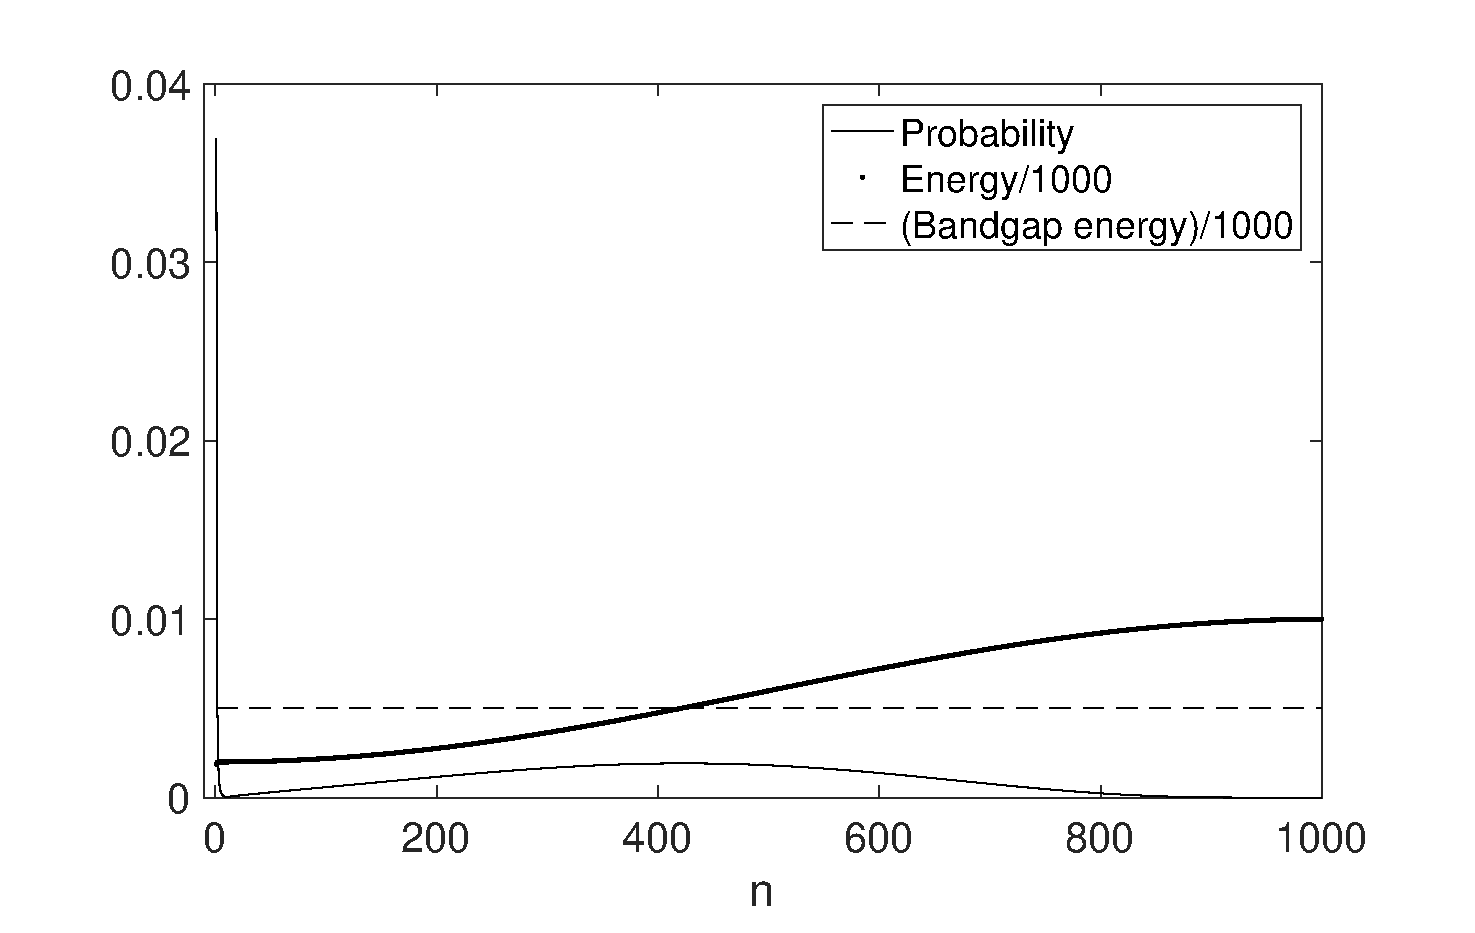
\includegraphics[width=0.7\textwidth]{fig/ExcitonStateU1.eps}
      \caption{The exciton energies and the lowest energy exciton probability plotted as a function of the distance between the electron and holes in unit cells. Shown is also the bandgap energy. For U = 1.} 
      \label{fig:U1}
  \end{figure}
\begin{figure}[!ht]
      \centering
      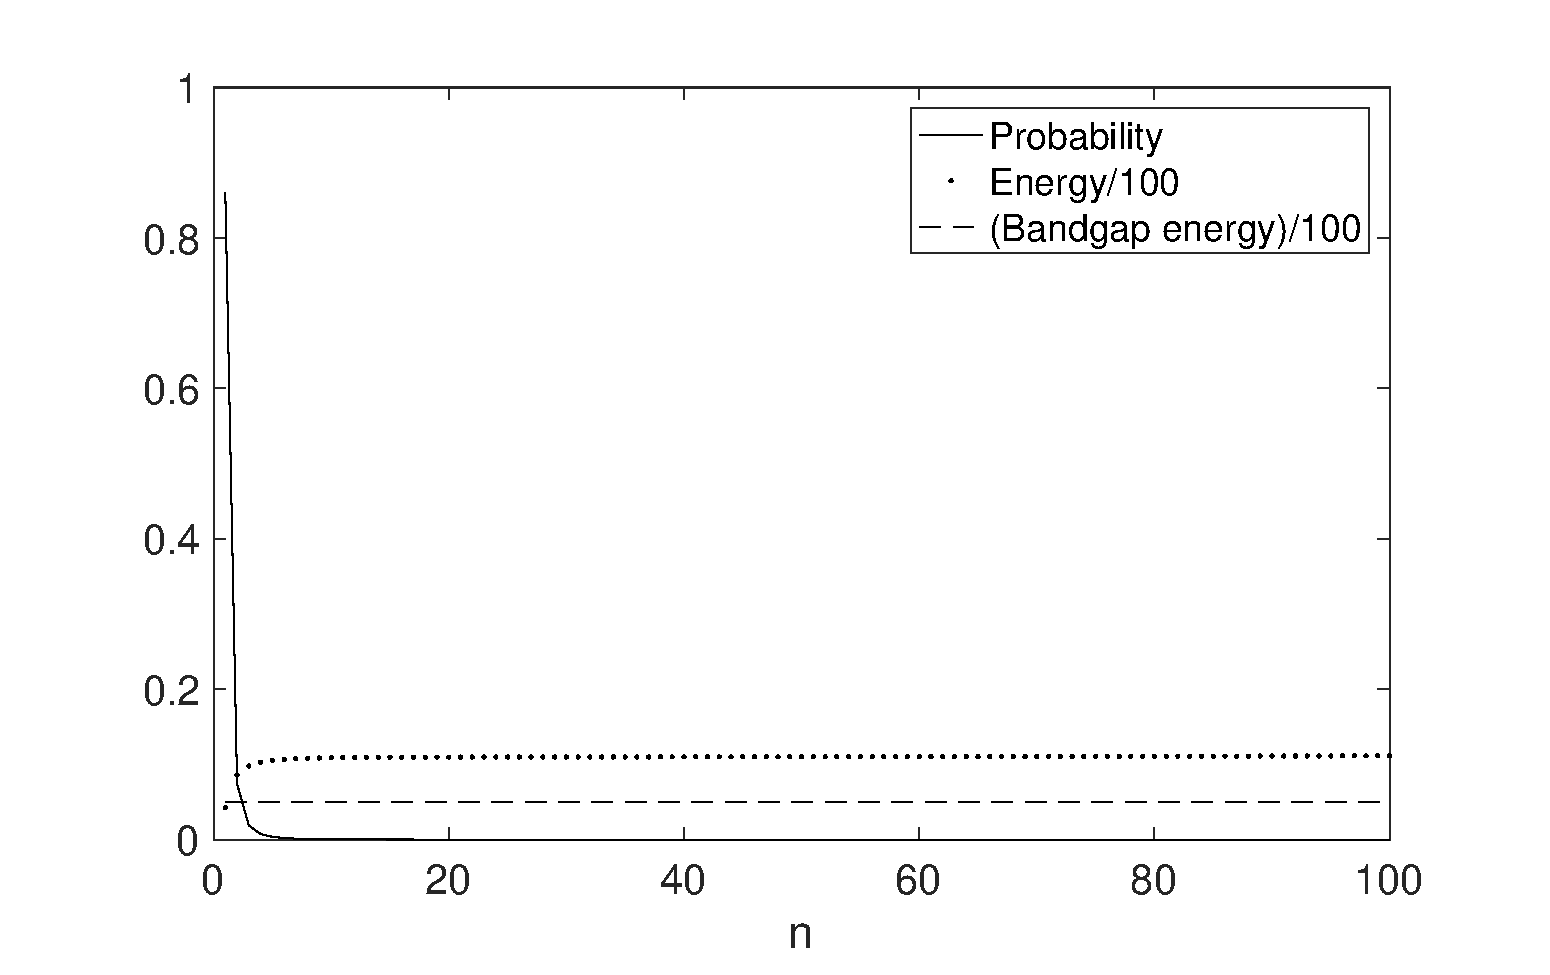
\includegraphics[width = 0.7\linewidth]{fig/ExcitonStateU10.eps}
      \caption{The exciton energies and the lowest energy exciton probability plotted as a function of the distance between the electron and holes in unit cells. Shown is also the bandgap energy. For U = 10.}
      \label{fig:U10}
\end{figure}

\begin{exercise}
Calculate (numerically) and plot the wave function $F_1(n)$ for the lowest lying excition.
\end{exercise}
\begin{solution}

\end{solution}